%%%%%%%%%%%%%%%%%%%%%%%%%%%%%%%%%%%%%%%%%%%%%%%%%%%%%%%%%%%%%%%%%%%%%%%%%%%%
% AGUJournalTemplate.tex: this template file is for articles formatted with LaTeX
%
% This file includes commands and instructions
% given in the order necessary to produce a final output that will
% satisfy AGU requirements, including customized APA reference formatting.
%
% You may copy this file and give it your
% article name, and enter your text.
%
% guidelines and troubleshooting are here: 

%% To submit your paper:
\documentclass[draft]{agujournal2019}
\usepackage{url} %this package should fix any errors with URLs in refs.
\usepackage{lineno}
\usepackage[inline]{trackchanges} %for better track changes. finalnew option will compile document with changes incorporated.
\usepackage{soul}
\linenumbers

% Julia's packages
\usepackage{amssymb,amsmath,mathtools,amsthm,amscd,mathrsfs,graphicx,color} % Basics
\usepackage[cmtip,all,matrix,arrow,tips,curve]{xy} % For drawing diagrams
\usepackage[active]{srcltx} % Allows jumping from code <-> pdf
\usepackage{anyfontsize} % Fixes issues with font size
\usepackage{cancel} % Provides cancellation symbol in equations
\usepackage{verbatim} % Provides comment environment and printing of literal text
\usepackage{bm} % For bold symbols
\usepackage{wrapfig} % Allows text to wrap around figures
\usepackage{float} % Allows forcing figure positions
\usepackage{tikz} % Allows creation of native figures
\usepackage{hhline} % Provides double hlines for tables
\usepackage{enumitem} % Allows for [nosep] and [noitemsep] in enumerate environment
\usepackage[final]{showlabels} % Show/hide labels
  % [inline] [final]

% Julia's commands
\newcommand{\todo}[1]{\textcolor{red}{\textbf{[TODO: #1}]}}
\newcommand{\e}[1]{\cdot 10^{#1}}
\newcommand{\del}{\bm{\nabla}}
\newcommand{\cross}{\times}
\newcommand{\mathdeg}{^\circ}
\newcommand{\ugy}{$\mu$Gy}

%%%%%%%
% As of 2018 we recommend use of the TrackChanges package to mark revisions.
% The trackchanges package adds five new LaTeX commands:
%
%  \note[editor]{The note}
%  \annote[editor]{Text to annotate}{The note}
%  \add[editor]{Text to add}
%  \remove[editor]{Text to remove}
%  \change[editor]{Text to remove}{Text to add}
%
% complete documentation is here: http://trackchanges.sourceforge.net/
%%%%%%%

\draftfalse

%% Enter journal name below.
%% Choose from this list of Journals:
%
% JGR: Atmospheres
% JGR: Biogeosciences
% JGR: Earth Surface
% JGR: Oceans
% JGR: Planets
% JGR: Solid Earth
% JGR: Space Physics
% Global Biogeochemical Cycles
% Geophysical Research Letters
% Paleoceanography and Paleoclimatology
% Radio Science
% Reviews of Geophysics
% Tectonics
% Space Weather
% Water Resources Research
% Geochemistry, Geophysics, Geosystems
% Journal of Advances in Modeling Earth Systems (JAMES)
% Earth's Future
% Earth and Space Science
% Geohealth
%
% ie, \journalname{Water Resources Research}

\journalname{Space Weather}

\hfuzz=100pt % Stop giving me overfull hbox errors for every single line that wraps!!!

\begin{document}

%%%%%%%%%%%%%%%%%%%%%%%%%%%%%%%%%%%%%%%%%%%%%%%
%  TITLE
%
% (A title should be specific, informative, and brief. Use
% abbreviations only if they are defined in the abstract. Titles that
% start with general keywords then specific terms are optimized in
% searches)
%
%%%%%%%%%%%%%%%%%%%%%%%%%%%%%%%%%%%%%%%%%%%%%%%

\title{On the Role of Electron Precipitation in Excess Radiation Doses Measured at Aviation Altitudes}

%%%%%%%%%%%%%%%%%%%%%%%%%%%%%%%%%%%%%%%%%%%%%%%
%
%  AUTHORS AND AFFILIATIONS
%
%%%%%%%%%%%%%%%%%%%%%%%%%%%%%%%%%%%%%%%%%%%%%%%

% Authors are individuals who have significantly contributed to the
% research and preparation of the article. Group authors are allowed, if
% each author in the group is separately identified in an appendix.)

% List authors by first name or initial followed by last name and
% separated by commas. Use \affil{} to number affiliations, and
% \thanks{} for author notes.
% Additional author notes should be indicated with \thanks{} (for
% example, for current addresses).

% Example: \authors{A. B. Author\affil{1}\thanks{Current address, Antartica}, B. C. Author\affil{2,3}, and D. E.
% Author\affil{3,4}\thanks{Also funded by Monsanto.}}

\authors{Julia Luna Claxton\affil{1}, Robert Marshall\affil{1}}

\affiliation{1}{Ann and H. J. Smead Department of Aerospace Engineering Sciences, University of Colorado Boulder}
\affiliation{1}{Boulder, CO, USA}

% Corresponding author mailing address and e-mail address:
% (include name and email addresses of the corresponding author.  More
% than one corresponding author is allowed in this LaTeX file and for
% publication; but only one corresponding author is allowed in our
% editorial system.)

% Example: \correspondingauthor{First and Last Name}{email@address.edu}
\correspondingauthor{Julia Luna Claxton}{julia.claxton@colorado.edu}



%%%%%%%%%%%%%%%%%%%%%%%%%%%%%%%%%%%%%%%%%%%%%%%
% KEY POINTS
%%%%%%%%%%%%%%%%%%%%%%%%%%%%%%%%%%%%%%%%%%%%%%%
%  List up to three key points (at least one is required)
%  Key Points summarize the main points and conclusions of the article
%  Each must be 140 characters or fewer with no special characters or punctuation and must be complete sentences

% Example:
% \begin{keypoints}
% \item	List up to three key points (at least one is required)
% \item	Key Points summarize the main points and conclusions of the article
% \item	Each must be 140 characters or fewer with no special characters or punctuation and must be complete sentences
% \end{keypoints}

\begin{keypoints}
  \item An existing model of particle precipitation is used to predict radiation dose rates due to galactic cosmic rays (GCRs) and relativistic electron precipitation (REP).
  \item Our predictions of GCR dose rates are in statistical agreement with aircraft dosimetry data, but do not explain a small population of higher dose rates.
  \item We model REP-induced dose rates and find that they are unlikely to account for the difference between GCR modeling and aircraft dosimetry data.
\end{keypoints}

%%%%%%%%%%%%%%%%%%%%%%%%%%%%%%%%%%%%%%%%%%%%%%%
%
%  ABSTRACT and PLAIN LANGUAGE SUMMARY
%
% A good Abstract will begin with a short description of the problem
% being addressed, briefly describe the new data or analyses, then
% briefly states the main conclusion(s) and how they are supported and
% uncertainties.

% The Plain Language Summary should be written for a broad audience,
% including journalists and the science-interested public, that will not have 
% a background in your field.
%
% A Plain Language Summary is required in GRL, JGR: Planets, JGR: Biogeosciences,
% JGR: Oceans, G-Cubed, Reviews of Geophysics, and JAMES.
% see http://sharingscience.agu.org/creating-plain-language-summary/)
%
%%%%%%%%%%%%%%%%%%%%%%%%%%%%%%%%%%%%%%%%%%%%%%%

%% \begin{abstract} starts the second page

\begin{abstract}
Radiation from space in the form of galactic cosmic rays (GCRs) generates a persistent background of ionizing radiation in Earth's atmosphere. The dose rate of ionizing radiation due to GCRs increases from sea level to aviation altitudes. The Nowcast of Aerospace Ionizing RAdiation System (NAIRAS) model is the state-of-the-art model for predicting radiation dose rates at aviation altitudes and is used to limit doses to aircrew and passengers. However, dosimetry data from the Automated Radiation Measurements for Aerospace Safety (ARMAS) system flown on commercial aircraft have revealed dose rates at aviation altitudes greater than predicted by NAIRAS. One theory, supported by correlation analyses, posits that these so-called excess dose rates are caused by relativistic electron precipitation (REP) driven by hiss waves in the inner magnetosphere. In this work, we use a validated Monte Carlo model of particle transport through the atmosphere in combination with GCR measurements from low Earth orbit (LEO) to attempt to explain the ARMAS dose rate measurements with GCRs alone. We find that our predicted GCR dose rates are in statistical agreement with the ARMAS data, but still underestimate the dose rates for some events. We then simulate REP using electron measurements from LEO and find that REP can only explain up to about $3\%$ of the difference between GCR dose rates and ARMAS data in the most extreme cases. With support from previous literature, we conclude that REP is unlikely to be the source of the discrepancies between GCR dose rate predictions and ARMAS measurements.
\end{abstract}

\section*{Plain Language Summary}
% Here are instructions on writing a Plain Language Summary: 
% https://www.agu.org/Share-and-Advocate/Share/Community/Plain-language-summary
Background radiation levels are higher in aircraft than they are on the ground due to their proximity to space. The airline industry relies on advanced computer simulations to predict high-altitude radiation levels to limit radiation doses to aircrew and passengers. However, measurements of radiation taken on airplanes have revealed occasional radiation spikes that these simulations did not predict. The reason for these spikes is currently unknown. One leading theory says that the spikes could be caused by a well-known process where natural radio waves in space divert extra radiation from space to Earth. In this paper, we test that theory using our own computer simulation and data from radiation detectors in space. We find that radiation sent into Earth's atmosphere by radio waves is unlikely to be the reason for the spikes and that further investigation is required to determine why our radiation predictions do not match the aircraft measurements.

\section{Introduction}
Relativistic charged particles from space are a major source of radiation on Earth. These particles collide with the atmosphere and create showers of secondary particles that can propagate down to tens of kilometers above sea level and even reach the ground. Exposure to these energetic particles and their secondary showers can ionize human tissue. Lifetime exposure to ionizing radiation in conjunction with peak dose rate is a major predictive factor in the development of cancerous and non-cancerous adverse health effects \cite{lowe2022, shah2014}. At commercial aviation altitudes (approximately $8$ to $11$~km above sea level), ionizing radiation doses from spaceborne particles are elevated compared to sea level due to a reduction in atmospheric shielding of these particles. Therefore, frequent fliers and aircrew are exposed to higher lifetime radiation exposure and peak dose rates than people on the ground. We thus require accurate models of radiation dose rates as a function of altitude to limit radiation doses to aircrew and passengers and ensure human safety. The industry standard for modeling ionizing radiation dose rates at aviation altitudes is the Nowcast of Aerospace Ionizing RAdiation System (NAIRAS) model maintained by NASA \cite{mertens2013}. NAIRAS predicts background radiation doses due to galactic cosmic rays (GCRs) and solar energetic particles (SEPs).

The Automated Radiation Measurements for Aerospace Safety (ARMAS) system is a set of dosimeters that have been flown in the last decade on commercial aircraft to monitor the radiation environment at aviation altitudes \cite{tobiska2016}. Data from the ARMAS system has revealed sporadic dose rate spikes at aviation altitudes, sometimes in excess of two times the NAIRAS-predicted dose rate \cite{tobiska2016, tobiska2018}. The cause of these excess doses is unknown, and a number of theories have emerged to explain them. One theory posits that relativistic electron precipitation (REP) may cause these excess doses. While energetic electrons cannot reach aviation altitudes, their secondary particles can, in particular X-rays and gamma rays produced by bremsstrahlung in the atmosphere. This theory is supported by correlation analyses \cite{aryan2023, aryan2025a, aryan2025b}, but has not yet been physically modeled to constrain the potential contribution of electron precipitation to excess dose rates.

In this work, we use energetic electron data collected from low Earth orbit (LEO) in combination with a validated particle precipitation model to quantify the contribution of electron precipitation to radiation dose rates at aviation altitudes. First, we use galactic cosmic ray (GCR) data measured in LEO in combination with a validated model of energetic particle precipitation to attempt to explain the ARMAS dose rates with GCRs alone. We then compare our model estimates to ARMAS data and identify cases of excess dose rates. Next, we forward model precipitating electron fluxes measured from LEO through the atmosphere to predict the radiation dose rate caused by radiation belt electron precipitation. We then compare the electron-induced dose rate to the excess dose rates between our GCR modeling and ARMAS. We find that REP-induced dose rates are unlikely to explain the excess dose rates, in agreement with previous literature.

\section{Background}
There are two well-known sources of background radiation doses at aviation altitudes: SEPs and GCRs \cite{mertens2013}. The state-of-the-art model for predicting radiation doses across the Earth's atmosphere, NAIRAS \cite{mertens2013}, accounts for both of these radiation types. NAIRAS parameterizes incoming GCR spectra using high-latitude neutron counts. Neutrons are produced as a cascade product from GCRs incident on the atmosphere, and thus their detection rate at the ground serves as an indirect measure of GCR incidence. NAIRAS then propagates the derived GCR spectrum through the heliosphere, magnetosphere, and atmosphere to produce dose rate predictions. We do not discuss SEP contributions to dose rate in this paper, as there are no ARMAS data records correlated with SEP events. NAIRAS, currently in version 3, was validated with aircraft dosimeter data from the RAD-X balloon campaign showing agreement within the measurement uncertainty of $\pm 30\%$. In this work, we utilize NAIRAS version 3 values that are provided with ARMAS data.

\citeA{tobiska2016} reported measurements from the ARMAS system revealing unexpected dose rate spikes at aviation altitudes, in some cases doubling NAIRAS version 2 predictions. These elevated dose rates were observed between L-shells of $1.5$ and $5$. This L-shell range led the authors to speculate that the dose rate spikes could be caused by relativistic electron precipitation (REP) driven by electromagnetic ion-cyclotron (EMIC) waves in the outer radiation belt.
  % tobiska2016: "Another intriguing suggestion is that this radiation enhancement could be from energetic electrons or O+ precipitating into higher altitudes from the outer radiation belt due to electromagnetic ion cyclotron (EMIC) waves (A. Halford, private communication, 2016). In addition, backscattered albedo electrons (J. Adams, private communication, 2016) may contribute radiation at higher altitudes than this flight as well as gamma rays from large storm or hurricane lightning, and sprite events may contribute to a radiation field enhancement. The Case 2 higher dose rates did not occur at altitudes where albedo electrons are expected, nor was the flight in the vicinity of a large tropospheric storm"
In \citeA{tobiska2018}, the excess dose rates recorded by ARMAS were posited to be caused by secondary bremsstrahlung X-rays generated by relativistic electron precipitation, and the ARMAS database was released publicly for further investigation.
  % "A particular feature of the ARMAS database is that measurements for L shells between 1.5 and 5 contain an additional contribution of radiation above the GCR background. These additional radiation levels have been carefully studied in over 50 cases and are not instrument artifacts whose characteristics have been previously described (Tobiska et al., 2016). A common characteristic of these enhanced radiation event periods is that the radiation levels during flight start at the GCR background level, rise to almost a factor of 2 higher, and then return to background GCR levels within less than an hour. This is consistent with flight through a secondary, Bremstrahlung γ ray beam."

If these excess dose rates are caused by electron precipitation from the radiation belts, then one would expect to find a correlation between excess dose rates and well-known drivers of REP. This led to a number of correlation studies investigating the idea that the excess dose rates could be caused by REP. In the first of these studies, \citeA{aryan2023} conducted a correlation analysis between excess dose rates and magnetospheric wave power during magnetic conjunctions between the Van Allen Probes and ARMAS ($\Delta$L $< 1$, $\Delta$MLT $< 1$~hr). They parameterized wave power by the power spectral density (PSD) in characteristic frequency bands for EMIC, hiss, chorus, and generalized high-frequency waves. They found a correlation between PSD in a frequency band associated with hiss ($100$~Hz to $2$~kHz) and excess dose rate, as well as a weaker correlation between PSD in a chorus-associated band ($0.1$x to $1$x the electron gyrofrequency) and excess dose rate. They concluded that hiss-driven precipitation may play a significant role in the generation of excess dose rates.

Continuing this work, \citeA{aryan2025a} and \citeA{aryan2025b} performed cross-correlation studies showing that the correlation between hiss-associated PSD and excess dose rate is strongest for close conjunctions in L-shell and magnetic local time (MLT) and decreases with increasing conjunction distance and time. Furthermore, they found a less rapid dropoff in correlation coefficient for eastward changes in MLT compared to westward changes, consistent with electron drift. However, their sampling distribution was heavily biased towards the post-noon and pre-midnight MLT sectors where hiss waves are primarily observed \cite{dong2024, hartley2018, li2015}, with a total of only $7$ datapoints in the 0000 to 0600 sector. They concluded that the excess dose rates measured by ARMAS were most likely caused by hiss-driven electron precipitation.

Despite the growing body of correlation studies between drivers of electron precipitation and excess dose rate, few modeling studies have been performed to quantitatively constrain the dose rates that electron precipitation could induce at aviation altitudes. \citeA{xu2021} studied the dose rates induced by monoenergetic beams of electrons propagated through a simulated atmosphere using the Energetic Precipitation Monte Carlo (EPMC) model \cite{lehtinen1999} in conjunction with the Monte Carlo model for Photons (MCP) \cite{xu2012}. They predicted that a precipitating flux of $10^8$~electrons$~\cdot~$m$^{-2}~\cdot~$s$^{-1}$ of $10$~MeV electrons would induce a dose rate of just over $0.1$~$\mu$Sv/hr at $11$~km. The quality factor converting Gy to Sv in silicon is approximately $2$, meaning they predicted an induced dose rate of approximately $0.05$~{\ugy}/hr in a silicon detector at aviation altitudes. They also predicted that precipitating electrons with energies less than $\sim 1$~MeV do not meaningfully contribute to dose rates at aviation altitudes. However, their work did not model realistic energy distributions of energetic electrons, instead reporting the induced dose rates for single monoenergetic beams.

\citeA{mcmurchie2022} used the \citeA{xu2021} parameterization of REP-induced dose rates to predict dose rates due to precipitating electron spectra derived from the POES constellation. They conducted three case studies corresponding to storm time, moderate disturbance, and quiet time. They predicted that electron precipitation explained up to $0.035\%$ of the total (not excess) ARMAS-measured dose rate during the storm case, $3.66\%$ of the total dose rate in the moderate disturbance case, and $0.015\%$ of the total dose rate in the quiet case. However, the precipitating electron spectra that they used in their modeling were limited due to the coarse energy resolution of the POES detectors, the limited coverage of high-energy electrons in those detectors, and contamination between the $0\mathdeg$ and $90\mathdeg$ telescopes \cite{selesnick2020}.

In this work, we use a validated Monte Carlo model in conjunction with the highest-quality measurements of precipitating electrons currently available to quantitatively constrain the contribution of electron precipitation to the unexplained excess dose rates measured by ARMAS. To our knowledge, this is the first study to directly compare simulated dose rates using high-quality in-situ measurements of precipitating particles (including protons, alpha particles, and electrons) to the excess dose rates recorded by ARMAS. This work is thus the most direct evaluation to date of the hypothesis that REP is responsible for the ARMAS excess dose rates.

% \cite{aryan2023} the bortnik hiss correlation paper. RBSP EMFISIS for wave data. finds no EMIC PSD correlation. finds hiss PSD correlation. finds weak hiss PSD correlation.

% \cite{aryan2025a} basically the same as last paper but with some time/L shift analysis. finds the same hiss correlation that is localized in L and MLT. shows L-MLT coverage that extremely heavily favors the post-noon sector.
  
% \cite{aryan2025b} time shift analysis paper, finds strong correlation for small L and MLT shifts, with eastward MLT drift.

% NAIRAS https://agupubs.onlinelibrary.wiley.com/doi/10.1002/swe.20100

\section{Model Description: SEPIIDA}
In this work, we utilize the Simulation of Energetic Particle Incidence, Ionization, and Dynamics in an Atmosphere (SEPIIDA) model. SEPIIDA is a modification of the model introduced in \citeA{berland2023}. SEPIIDA utilizes the Geant4 simulation package developed by CERN \cite{geant4} to simulate a $1000$~km MSIS atmosphere divided into $1$~km slabs. Particles of arbitrary species, energy, and direction can be injected at any point in the simulated atmosphere and traced through their lifetime. SEPIIDA accounts for secondary cascade processes, including electron production via ionization, photoelectron production, and pair production, as well as pair annihilation, bremsstrahlung photon production, and Compton scattering \cite{berland2023}. Note that this is not an exhaustive list of processes included in the SEPIIDA model. For more information, see the Geant4 documentation describing the QBBC physics list \cite{qbbc-docs}. SEPIIDA-simulated electron backscatter has been validated using data from low Earth orbit in \citeA{claxton2026accepted}. SEPIIDA features a 3-dimensional vector dipolar magnetic field model, providing magnetic mirroring without the use of a nonphysical external mirroring force. For this work, we configured SEPIIDA to operate at a magnetic latitude of $45\mathdeg$, corresponding roughly to the magnetic latitude of the continental United States where the majority of ARMAS data were recorded. The magnetic dip angle at this latitude at an altitude of $450$~km in our simulation is $26.6\mathdeg$ from vertical-down.

\subsection{Simulated Dose Rate Calculation}
\label{section:model:doserate_conversion}
We begin by attempting to explain the ARMAS dose rate measurements using an upper-bound estimate of GCR-induced dose rates. In addition to validating the SEPIIDA model, these simulations provide a picture of data-driven dose rates produced by GCRs and their day-to-day variability based on direct measurements from LEO.

To model the dose rate induced by GCRs at aviation altitudes, we needed to calculate the dose rate induced by a given set of precipitating particles. For protons, electrons, and alpha particles, we utilized the fact that particle flux multiplied by stopping power in a material of interest (e.g. silicon) yields a dose rate in that material. The cumulative dose rate induced by protons, electrons, and alpha particles at altitude $h$ is given by
%
\begin{equation}
  \text{DR}_{\text{p}^+,\text{e}^-,\alpha}(h) = \sum_i \sum_E \Phi_i(E,h) \cdot \text{S}_i(E,h),
\end{equation}
%
\noindent where $i$ represents particle species, $E$ is the energy of an incident particle, $\Phi_i(E)$ is the flux of species $i$ at energy $E$, $S$ is the stopping power of silicon for species $i$ at energy $E$, and DR$_{\text{p}^+,\text{e}^-,\alpha}$ is the resultant cumulative dose rate in silicon due to these particles.

% https://physics.nist.gov/PhysRefData/XrayMassCoef/chap3.html
High-energy photons are another important source of ionizing radiation doses. Since stopping power is not defined for photons, we estimated the energy deposited in a silicon detector by photons using the X-ray mass energy-absorption coefficient $\mu_\text{en}$. For a given photon, $\mu_\text{en}$ multiplied by the incident photon energy yields the net energy deposition in a target material per unit flux accounting for both energy deposition by the original photon and energy losses via re-radiation of secondaries. Multiplying by a photon flux thus yields the dose rate in silicon due to photons. Thus, for a given flux of photons $\Phi_\gamma$, the photon contribution to dose rate (DR$_\gamma$) is
%
\begin{equation}
  \text{DR}_\gamma(h) = \sum_E \Phi_\gamma(E,h) \cdot E \cdot \mu_\text{en}(E),
\end{equation}
%
\noindent and the total dose rate (DR) is
%
\begin{equation}
  \text{DR}(h) = \text{DR}_{\text{p}^+,\text{e}^-,\alpha}(h) + \text{DR}_\gamma(h).
\end{equation}
%
Stopping power tables were sourced from NIST for protons ($1$~keV to $10$~GeV), electrons ($10$~keV to $1$~GeV), and alphas ($1$~keV to $1$~GeV) \cite{nist-stoppingpower}. X-ray mass energy-absorption coefficients were sourced from NIST for photons between $1$~keV and $20$~MeV \cite{nist-xrayattenuation}. The value of $\mu_\text{en}$ for photons above $20$~MeV was taken as the value at $20$~MeV, as $\mu_\text{en}$ does not change significantly with energy above $\sim 5$~MeV in the NIST database. This extrapolation added approximately $0.6$~{\ugy}/hr to our predicted GCR dose rates at aviation altitudes. The stopping power and X-ray mass energy-absorption coefficient values used in this work are shown in Figure \ref{figure:stopping_power}.

\begin{figure}[H]
  \centering
  \noindent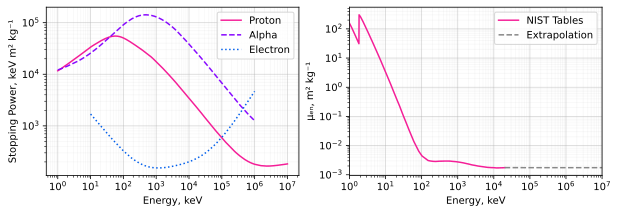
\includegraphics[width=\textwidth]{figures/stopping_power.png}
  \caption{
    Stopping power (left) and X-ray mass energy-absorption coefficient (right) as a function of energy used in this work.
  }
  \label{figure:stopping_power}
\end{figure}

Since the calculation of dose rate is species- and energy-dependent, we need to record an energy spectrum for every species of interest at every location where we want to calculate a dose rate in our simulation. Since we are interested in the altitude profile of EPP-induced dose rates, we configure SEPIIDA to record the energy spectrum of all electrons, protons, alphas, and photons passing through a set of recording altitudes. These recording altitudes are spaced from sea level to $100$~km altitude in $1$~km increments. After a simulation run is completed, the counts recorded in every energy bin at each recording altitude are divided by the total number of input particles. This division produces a normalized response table giving the number of counts of a given particle that are produced by one precipitating primary particle over the energies and altitudes of interest. An example of these normalized response spectra is shown in Figure \ref{figure:example_histograms}. The spectra shown are the response to a monoenergetic input beam of $10^5$ protons each with an energy of $1.1$~GeV injected into the simulation at $450$~km with an initial velocity randomly sampled from an isotropically downgoing distribution. Secondary alpha fluxes are negligible and are not shown in the figure. The primary protons are evident as the white line in the leftmost panel, with the primary energy decreasing at low altitudes. The $511$~keV photon line due to pair annihilation is evident in the rightmost panel.

\begin{figure}[H]
  \centering
  \noindent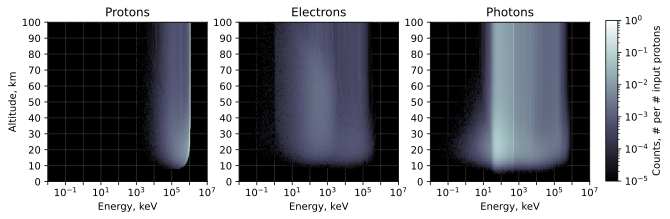
\includegraphics[width=\textwidth]{figures/example_histograms.pdf}
  \caption{
    Example simulated energy spectra as a function of altitude for protons (left), electrons (center), and photons (right). These spectra are the response to an input beam of $10^5$ protons at $1.1$~GeV injected with isotropic downgoing incidence into an MSIS atmosphere at $450$~km.
  }
  \label{figure:example_histograms}
\end{figure}

\section{Galactic Cosmic Ray Dose Rates}
\label{section:gcrs}
While the primary goal of this study is to constrain dose rates due to REP, we first attempt to explain the ARMAS-measured dose rates with GCRs alone. Since NAIRAS estimates of GCR dose rates do not explain the ARMAS dose rates, we seek to model upper-bound GCR dose rates using our own modeling. To perform this modeling, we utilize data from the Alpha Magnetic Spectrometer (AMS-02) on board the International Space Station (ISS) \cite{ams02}. AMS-02 measures GCR energy spectra at a daily cadence for a number of particle species. In this work, we consider the proton and alpha particle contribution to dose rate. AMS-02 measures GCR protons between $0.4$~GeV and $99$~GeV and alpha particles between $1.3$~GeV and $135.7$~GeV.

To convert a spectrum measured by AMS-02 into a dose rate profile, we used the SEPIIDA model to inject a series of monoenergetic proton and alpha beams into a simulated atmosphere. Each beam had an energy corresponding to the mean energy of an AMS-02 energy channel. We injected these beams into our simulation with an initial velocity randomly selected from an isotropically downgoing distribution. Each beam consisted of $10^5$ particles. As described in Section \ref{section:model:doserate_conversion}, energy spectra of primary particles and cascade products were recorded along the atmospheric column for each beam. These spectra provide a basis set of atmospheric responses to protons and alpha particles. The response tables were saved to a datafile for later lookup. Performing a sum of these lookup tables weighted by the flux measured by AMS-02 thus provides a composite atmospheric response for a given AMS-02 spectrum.

To calculate lookup table weights, we first integrate a given AMS-02 spectrum over solid angle. This solid angle integration is performed over a full $2\pi$ hemisphere, thus assuming an isotropic distribution of incoming GCRs. In reality, the solid angle over which GCRs arrive at LEO is rigidity-dependent and smaller than $2\pi$ for particles with rigidities below approximately $10$~GV \cite{chen2025}. The isotropic hemisphere assumption likely overestimates the flux of lower-rigidity particles, thus increasing our GCR dose rate predictions. This assumption was made for ease of calculation and in pursuit of our goal of finding an upper-bound GCR dose rate.

After solid angle integration, we perform a trapezoidal integration over energy with bounds corresponding to the midpoints between the beam energies we injected into the SEPIIDA simulation. This step produces a flux in units of particles~$\cdot~\text{m}^{-2}~\text{ s}^{-1}$. The atmospheric response table corresponding to each beam was then multiplied by the integrated flux derived from AMS-02 for that beam. The response due to each beam is then summed for every species, creating composite energy spectra at every $1$-kilometer altitude step between $0$~km and $100$~km above sea level. The resulting dose rate is then derived from these spectra following the process described in Section \ref{section:model:doserate_conversion}. An example spectrum recorded by AMS-02 and the associated dose rate calculated from our model are shown in Figure \ref{figure:gcr_spectrum}. The dose rate includes the contributions of protons and alpha particles.

\begin{figure}[H]
  \centering
  \noindent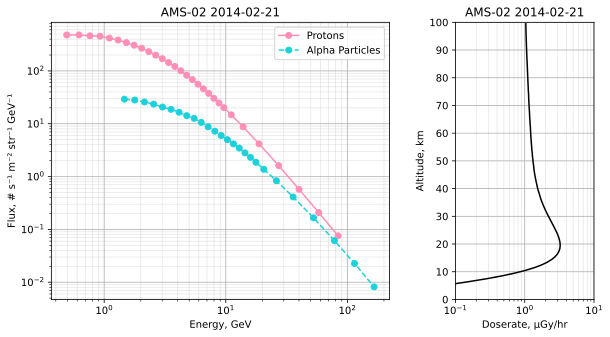
\includegraphics[width=\textwidth]{figures/gcr_spectrum.pdf}
  \caption{
      Left: Example of a cosmic ray spectrum measured in low Earth orbit by AMS-02 for protons (solid pink line) and alpha particles (dashed blue line). Right: Dose rate in silicon as a function of altitude predicted by our model due to the AMS-02-measured spectrum.
  }
  \label{figure:gcr_spectrum}
\end{figure}

In Figure \ref{figure:case_studies}, we plot four example conjunctions showing a) agreement between SEPIIDA, NAIRAS, and ARMAS; b) disagreement between NAIRAS and ARMAS, but agreement between ARMAS and SEPIIDA; c) small excess dose rates in ARMAS above the SEPIIDA prediction; and d) large excess dose rates in ARMAS above the SEPIIDA prediction. Error bars on ARMAS data represent the $1\sigma$ uncertainty, which is $20\%$. SEPIIDA predictions of dose rate are derived from AMS-02 data recorded on the date of each panel. Note that AMS-02 data is provided at a daily cadence for the ISS's orbit at $51\mathdeg$ inclination, spanning a range of latitudes, while the ARMAS data is primarily limited to the mid-latitudes of the continental United States. Thus, the AMS-02 data experiences a wider range of cutoff rigidities than ARMAS and may record higher fluxes at low rigidities than ARMAS would experience, causing another potential overestimation of GCR dose rates. Once again, we accept this overestimation in order to determine if the excess dose rates can be explained by an upper-bound case for GCR dose rates.

\begin{figure}[H]
  \centering
  \noindent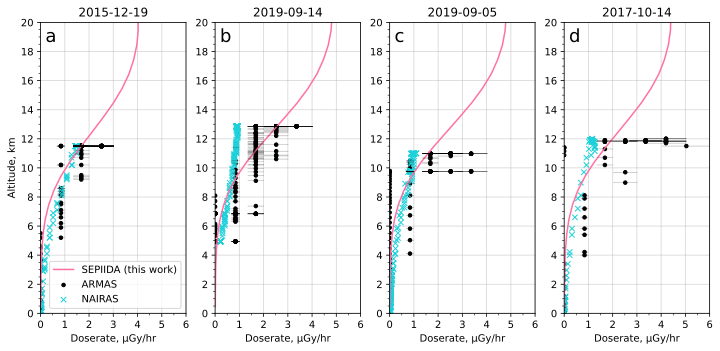
\includegraphics[width=\textwidth]{figures/case_studies.pdf}
  \caption{
      Four example conjunction dates between ARMAS and AMS-02 showing the ARMAS-measured dose rate (black dots), NAIRAS-predicted GCR dose rate (blue crosses), and our predicted GCR dose rate based on AMS-02 data (pink line).
  }
  \label{figure:case_studies}
\end{figure}

With the ability to compute a dose rate profile from an AMS-02 spectrum, we next compare our predicted GCR dose rates to ARMAS-measured dose rates for every day where AMS-02 and ARMAS both recorded data. For each day, we subtract our predicted GCR-induced dose rate from the ARMAS-measured dose rate to produce a residual dose rate. The GCR-induced dose rate was taken at the same altitude of each ARMAS data record. The results of this comparison are shown in Figure \ref{figure:armas_residuals}, along with the results of the same procedure using NAIRAS version 3 predictions of GCR dose rate for reference.

\begin{figure}[H]
  \centering
  \noindent\includegraphics[width=\textwidth]{figures/armas_residuals.pdf}
  \caption{
      Left: Residuals between our GCR dose rate predictions and ARMAS data for all conjunction dates with AMS-02. Right: Residuals between NAIRAS predictions and ARMAS data for the same set of dates.
  }
  \label{figure:armas_residuals}
\end{figure}

The results in Figure \ref{figure:armas_residuals} show that in general, our GCR dose rate estimations correctly predict the ARMAS data, with a preference to overestimating the ARMAS-measured dose rates more often than underestimating them. This tendency to overestimation indicates a systematic error consistent with our assumptions in favor of finding the upper-bound GCR dose rate. However, we note that the $3\sigma$ uncertainty of ARMAS is on the order of $\pm 1.5$~{\ugy}/hr at aviation cruising altitudes (Figure \ref{figure:case_studies}). Thus, some of these overestimate cases may be explained by uncertainty in the ARMAS measurements. However, there is a noticeable tail where we still underestimated the measured dose rates by up to $3$~{\ugy}/hr, despite our assumptions. Those dose rates cannot be reasonably explained by our modeling of GCRs.   

Having found a subset of ARMAS dose rates measurements that we cannot explain with GCRs alone, we next investigate the potential contribution of relativistic electron precipitation to these excess dose rates.

\section{Relativistic Electron Precipitation Dose Rates}
\label{section:rep}
To calculate the possible contribution of electron precipitation to dose rates at aviation altitudes, we require a realistic precipitating energy spectrum for energetic electrons. In this study, we use data from the Electron Losses and Fields INvestigation (ELFIN) mission \cite{angelopoulos2020} to provide realistic precipitating spectra. The twin ELFIN CubeSats, which flew from 2019 to 2022, measured precipitating, trapped, and backscattered electrons from low Earth orbit ($450$~km altitude, $93\mathdeg$ inclination) every $1.4$ seconds during its data collection periods. ELFIN measured electrons between $50$~keV and $7$~MeV in $16$ approximately logarithmically-spaced bins. An example of ELFIN data is shown in Figure \ref{figure:elfin_example_data}.

\begin{figure}[H]
  \centering
  \noindent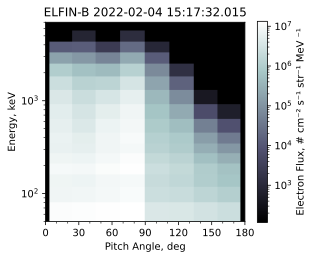
\includegraphics[width=0.6\textwidth]{figures/elfin_example_data.pdf}
  \caption{
    Example of one timestep ($1.4$~seconds) of ELFIN data. Data was recorded in the northern hemisphere with a loss cone angle of approximately $68\mathdeg$. 
  }
  \label{figure:elfin_example_data}
\end{figure}

We aim to find precipitating electron spectra recorded by ELFIN that are most likely to explain the excess dose rates measured by ARMAS. While correlation studies between excess dose rate and electron precipitation have largely focused on hiss-driven precipitation, the energy of precipitating electrons and their production of secondary particles is the primary factor that determines their penetration depth into the atmosphere rather than a specific wave driver \cite{berland2023, xu2021, marshall2018}. Therefore, harder precipitating spectra with higher fluxes above $1$~MeV induce higher dose rates at aviation altitudes regardless of the wave driver of the precipitation. We therefore look for the precipitating electron spectra measured by ELFIN that had the highest fluxes of high-energy electrons to try to explain the excess dose rates. To find these spectra, we sum the precipitating flux of supra-MeV electrons (i.e. $\geq 1$~MeV) for every half-spin (corresponding to a full sweep of the electron pitch angle distribution) of each ELFIN satellite over their lifetime. We then select spectra at the $90$th, $98$th, and $99.9$th percentile of precipitating supra-MeV fluxes for analysis. These spectra represent some of the most intense relativistic precipitation events ever recorded by the ELFIN mission. The date, time, and satellite for each spectrum is provided in Table \ref{table:rep:spectra_summary}, and the pitch angle-energy distribution of the $99.9$th percentile REP event is shown in Figure \ref{figure:elfin_example_data}.

\begin{table}[H]
  \centering
  \begin{tabular}{cccc}
    Percentile & Date (YYYY-MM-DD) & Time (UTC)   & Satellite \\
    \hline
    $99.9$     & 2022-02-04        & 15:17:32.015 & ELFIN-B   \\
    $98$       & 2021-11-07        & 02:12:46.867 & ELFIN-B   \\
    $90$       & 2020-10-22        & 23:04:22.315 & ELFIN-A  
  \end{tabular}
  \caption{
    Timestamps and satellite identification information for our selected ELFIN-measured spectra.
  }
  \label{table:rep:spectra_summary}
\end{table}

To predict the dose rates induced by our chosen precipitating electron spectra, we injected beams of field-aligned electrons into the SEPIIDA simulation corresponding to each of ELFIN's energy bins. The field-aligned assumption was made to reduce computation time and to maximize the penetration depth of primary electrons. The field-aligned assumption will thereby slightly overestimate the dose rate induced by electron precipitation. The resultant dose rates should thus be considered as upper bounds on the dose rate induced by each spectrum.

After injecting electron beams into SEPIIDA, the atmospheric response of each beam is weighted by the ELFIN-measured flux at that energy using the same procedure as with AMS-02 (Section \ref{section:gcrs}). The atmospheric response is then converted to a dose rate as described in Section \ref{section:model:doserate_conversion}. Our chosen REP spectra and their resulting upper-bound electron dose rates are shown in Figure \ref{figure:rep:electron_spectrum}.

\begin{figure}[H]
  \centering
  \noindent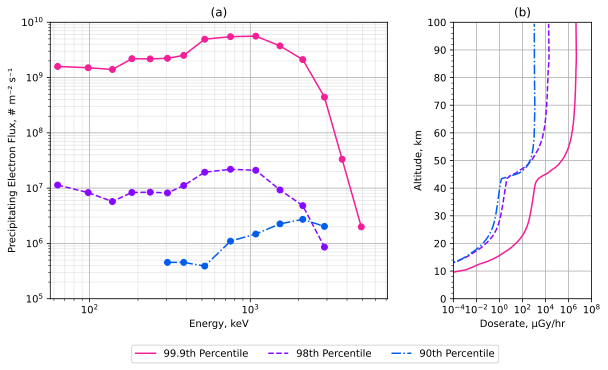
\includegraphics[width=\textwidth]{figures/electron_spectrum.pdf}
  \caption{
      (a) Precipitating electron spectra derived from ELFIN-measured datapoints at the $99.9$th (solid magenta line), $98$th (dashed purple line), and $90$th (dash-dotted blue line) percentile of supra-MeV electron precipitation events recorded by ELFIN. (b) Dose rate in a silicon detector due to each of the spectra in (a) as a function of altitude.
  }
  \label{figure:rep:electron_spectrum}
\end{figure}

We then compare our REP-induced dose rate to the excess dose rates we calculated in Section \ref{section:gcrs}. Figure \ref{figure:rep:excess_dose_comparison} shows the distribution of excess dose rates where ARMAS-measured dose rates exceeded our GCR predicted dose rates as a function of altitude. The predicted REP-induced dose rates induced by our selected events are overlaid on the same scale.

\begin{figure}[H]
  \centering
  \noindent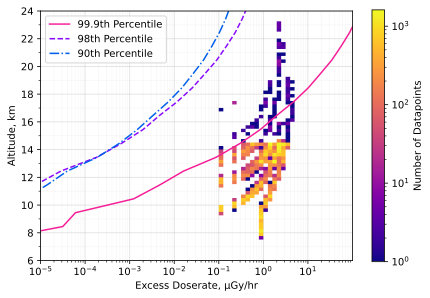
\includegraphics[width=.85\textwidth]{figures/excess_dose_comparison.pdf}
  \caption{
    Distribution of excess dose rates as a function of altitude (color) with overlaid curves showing the modeled dose rate due to the $99.9$th (solid magenta line), $98$th (dashed purple line), and $90$th (dash-dotted blue line) percentile of supra-MeV electron precipitation events recorded by ELFIN.
  }
  \label{figure:rep:excess_dose_comparison}
\end{figure}

Figure \ref{figure:rep:excess_dose_comparison} shows that the strongest relativistic electron precipitation ELFIN measured is not sufficient to explain the vast majority of excess dose rates observed by ARMAS, even with our assumptions to maximize the GCR component of total dose rate. The $99.9$th percentile REP-induced dose rate can only explain $0.5\%$ of the total number of excess dose rates recorded, and only at very high altitudes above $13$~km. Meanwhile, the $98$th and $90$th percentile events cannot account for any of the excess dose rate measurements. Often, the REP-induced dose rates are multiple orders of magnitude smaller than the excess dose rates measured by ARMAS.

\section{Discussion}
At each step in our analysis where there was uncertainty in the model inputs, we made the assumption in favor of giving REP the best chance possible to explain the excess dose rates. We assumed that GCRs were isotropically incoming over one hemisphere regardless of rigidity, overestimating the dose rate contribution of GCR particles with rigidities below $10$~GV. We also simulated incoming GCRs measured at lower cutoff rigidities than ARMAS experienced, allowing for potentially higher fluxes of low-rigidity particles than ARMAS would experience. Both of these assumptions increased our predicted GCR dose rates, thereby reducing the magnitude of the excess dose rates that needed to be explained by REP. Furthermore, when simulating REP, we assumed that precipitating electrons were exclusively field-aligned, maximizing their penetration depth into the atmosphere and thus their resultant dose rates. Finally, we chose to compare the excess dose rates to three cases of the most extreme REP events measured over the full lifetime of the ELFIN satellites.

However, despite these assumptions and choices, we found that the event corresponding to the $99.9$th percentile of REP strength measured by ELFIN could only explain a small number of excess dose rates at high altitudes. The $98$th percentile and below could not fully explain a single excess dose rate at any altitude. Furthermore, the excess dose rates explainable by the $99.9$th percentile REP event only occurred above $13$~km. At $11$~km (a more typical aviation altitude), the dose rate due to the $99.9$th percentile REP event explained only $0.1\%$ to $3\%$ of excess dose rate magnitudes, and the $98$th and $90$th percentile events explained less than $0.01\%$ of even the smallest excess dose rate magnitude. Moreover, our modeling predicts that REP can contribute only up to approximately $0.01$~{\ugy}/hr at aviation altitudes in the most extreme cases. We thus conclude that REP cannot reasonably explain the excess dose rates measured at aviation altitudes by ARMAS.

Previous modeling efforts also support this conclusion. As previously discussed, \citeA{xu2021} predicted that a flux of $10^8$~electrons$~\cdot~$m$^{-2}~\cdot~$s$^{-1}$ of $10$~MeV electrons, a flux orders of magnitude higher than typical observed electron fluxes at LEO, would induce a dose rate of just $0.05$~{\ugy}/hr at an altitude of $11$~km. Meanwhile, typical excess dose rates are on the order of $1$~{\ugy}/hr (Figure \ref{figure:rep:excess_dose_comparison}). Thus, their work predicts that an extreme flux of ultrarelativistic electrons could contribute only up to about $5\%$ of a typical excess dose rate. In the case studies presented by \citeA{mcmurchie2022}, the highest fraction of total (not excess) dose rate explained by REP was $3.66\%$. To explain the excess dose rates measured by ARMAS, REP-induced dose rates would have to make up about $10\%$ to $50\%$ of the total dose rate. The results of both of these studies suggest that REP is unlikely to be able to generate dose rates on the order of the observed excess dose rates.

We recognize the compelling correlation between hiss wave activity and excess dose rates presented in \citeA{aryan2025b}. The goal of this study is not to explain that correlation, but simply to quantitatively constrain the hypothesis that REP is responsible for that correlation. Between our analysis and previous literature, we believe it is unlikely that relativistic electron precipitation is the direct cause of the discrepancies between GCR dose rate predictions and dose rates measured by the ARMAS system.

\section{Conclusion}
In this work, we investigated the contribution of relativistic electron precipitation to radiation dose rates at aviation altitudes. We used the SEPIIDA model to forward model distributions of GCR ions and radiation belt electrons measured in-situ at the top of the atmosphere to calculate radiation dose rates through a column of atmosphere. We predicted that the dose rates due to REP cannot reasonably explain excess dose rates measured at aviation altitudes. Our results are in agreement with previous literature that used a different particle transport model. We therefore conclude that radiation belt electrons are unlikely to be the source of excess radiation doses at aviation altitudes, and moreover are unlikely to contribute any noticeable dose rate at those altitudes. Further investigation is required to determine the source of these excess dose rates and the reason for their correlation with magnetospheric hiss.

\section*{Open Research Section}
% This section MUST contain a statement that describes where the data supporting the conclusions can be obtained. Data cannot be listed as ''Available from authors'' or stored solely in supporting information. Citations to archived data should be included in your reference list. Wiley will publish it as a separate section on the paper’s page. Examples and complete information are here: https://www.agu.org/Publish with AGU/Publish/Author Resources/Data for Authors
ELFIN data \cite{angelopoulos2020} is available for free at \url{https://data.elfin.ucla.edu/ela/}. Geant4 \cite{geant4} is available for free from \url{https://geant4.web.cern.ch/download/11.3.2.html}. The SEPIIDA code used to generate lookup tables is available for free at \url{https://zenodo.org/records/18473011}. The atmospheric response lookup tables generated by the Geant4 simulation are available for free at \url{https://zenodo.org/records/18473108}. All code used to perform the analysis and generate figures for this paper is available for free at \url{https://zenodo.org/records/18473280} . Analysis was performed using the Julia coding language \cite{julia-language}, NumPy \cite{numpy}, SpacePy \cite{spacepy1, spacepy2}, and Matplotlib \cite{matplotlib}.

%\cite{code-citation-aviationg4}
%\cite{data-citation-tables}
%\cite{code-citation-mainrepo}

\section*{Conflict of Interest Declaration}
The authors declare there are no conflicts of interest for this manuscript.

\acknowledgments
%Enter acknowledgments here. This section is to acknowledge funding, thank colleagues, enter any secondary affiliations, and so on.
The authors acknowledge NASA award NNX14AN68G, NSF awards AGS-1242918 and AGS-2019950, and Vassilis Angelopoulos for use of ELFIN's EPD data. The authors thank Ethan Tsai for providing technical support with ELFIN data.

\bibliography{citations}

\end{document}